% !TeX encoding = UTF-8
%%%%%%%%%%%%%%%%%%%%%
%%%%% Anpassen! %%%%%
%%%%%%%%%%%%%%%%%%%%%
% Meta-Informationen 
\newcommand{\titel}{Community-basierte Wissensportale InDeKo.Navi Atlas}
\newcommand{\untertitel}{Installationsanleitung} 
\newcommand{\art}{Ausarbeitung}
\newcommand{\studiengang}{Wirtschaftsinformatik}
\newcommand{\autor}{Robin Helmedach, Konstantin Janzen, Friederike Lauterbach, Stephan Mende}
\newcommand{\email}{}
\newcommand{\matnr}{}
\newcommand{\institut}{Institut für Betriebswirtschaft und Wirtschaftsinformatik}
\newcommand{\arbeitsgruppe}{Arbeitsgruppe Informationssysteme und Unternehmensmodellierung}
\newcommand{\universitaet}{Universität Hildesheim \textbullet  Universitätsplatz 1 \textbullet  D-31134 Hildesheim}
\newcommand{\adresse}{\arbeitsgruppe  \textbullet  \institut \\ \universitaet}
\newcommand{\version}{Version 1.0}
\newcommand{\veranstaltung}{IT-Studienprojekt Master SoSe 2016 }

%%%%%%%%%%%%%%%%%%%%%%%%%%%%%%%%%%%%%%%%%%%%%
%% Diese Datei muss nicht angepasst werden %%
%%%%%%%%%%%%%%%%%%%%%%%%%%%%%%%%%%%%%%%%%%%%%
% v1.3
%Schriftgröße, ein- oder zweiseitig, Papierformat, Dokumententyp
\documentclass[12pt,oneside,a4paper,bibliography=totoc,listof=totoc,
	ngerman,
	parskip=half, % Abstand zwischen Absätzen (halbe Zeile)
	headings=normal, % Größe der Überschriften verkleinern
	]{scrartcl}

%Seitenränder
\usepackage[left=2cm,right=2cm,top=2.5cm,bottom=2.5cm]{geometry}

%Neue Deutsche Rechtschreibung und Umlaute
\usepackage[T1]{fontenc}
\usepackage[utf8]{inputenc}
\usepackage[ngerman]{babel}
\usepackage[babel,german=quotes]{csquotes}
\usepackage{lmodern}
\usepackage[right]{eurosym}

\usepackage{caption}
\usepackage{subcaption}

%Kopf- und Fußzeile
\usepackage{fancyhdr}
\pagestyle{fancy} 
\fancyhf{}


\usepackage{lastpage}

\usepackage{tabularx}
\newcolumntype{L}[1]{>{\raggedright\arraybackslash}p{#1}} % linksbündig mit Breitenangabe
\newcolumntype{C}[1]{>{\centering\arraybackslash}p{#1}} % zentriert mit Breitenangabe
\newcolumntype{R}[1]{>{\raggedleft\arraybackslash}p{#1}} % rechtsbündig mit Breitenangabe

%Kopfzeile links bzw. innen
%\fancyhead[L]{\name}

%Kopfzeile mittig
%\fancyhead[R]{\thepage}

%Kopfzeile rechts bzw. außen
%\fancyhead[L]{\rightmark}

%Fußzeile
%\cfoot{\thepage}

% Kopfzeile und Fußzeile einstellen
%\textsc{\lhead{\name, \matrikel}
%\chead{\veranstaltung\ \ubungsnr}
%\rhead{\today}
\cfoot{\thepage\ / \pageref*{LastPage}}

%Linie oben / unten
\renewcommand{\headrulewidth}{0pt}
%\renewcommand{\footrulewidth}{0.5pt}



%Hübbsche Schriften im PDF-Viewer
\usepackage{ae}
\usepackage{times}


\usepackage{booktabs}

\makeatletter
\@ifpackageloaded{tex4ht}{%
      \usepackage[dvips]{graphicx}
      \usepackage[tex4ht]{hyperref}
    }{%

% Brauchbare PDF-Links und Angaben im PDF-Header
% Graphiken
\usepackage[pdftex]{graphicx}
\usepackage[hyphens]{url}
\PassOptionsToPackage{hyphens}{url}
\usepackage[ %pdftex,
	raiselinks=true,%
	bookmarks=true,%
	colorlinks=true,% Gibt man keine gedruckte Version ab, sondern das PDF, sollte man erwägen diesesn Wert auf "true" zu ändern
	linkcolor=black, % einfache interne Verknüpfungen
	anchorcolor=black, % Ankertext
	citecolor=black, % Verweise auf Literaturverzeichniseinträge im Text
	filecolor=black, % Verknüpfungen, die lokale Dateien öffnen
	menucolor=black, % Acrobat-Menüpunkte
	urlcolor=blue, 
	bookmarksopenlevel=1,%
	bookmarksopen=true,%
	bookmarksnumbered=true,%
	hyperindex=true,% 
	hypertexnames=false, % zur korrekten Erstellung der Bookmarks
	plainpages=false,% correct hyperlinks
	pdfpagelabels=true,% view TeX pagenumber in PDF reader
%%  pdfborder={0 0 0.5}
	pdfauthor={\autor},
	pdfsubject={\titel},
	pdfkeywords={},
	pdftitle={\titel},
	linktocpage = false, % Seitenzahlen anstatt Text im Inhaltsverzeichnis verlinken
	pdfstartview=FitH
]{hyperref}

}
\makeatother
%Thumbnails im PDF
%\usepackage{thumbpdf}
%hübschere Tabellenabstände
\usepackage{booktabs}

%diverser mathematischer Kram
\usepackage{amsmath}
\usepackage{amsthm}
\usepackage{amssymb}
\usepackage{multirow}

% Zitierstil
%\usepackage[round]{natbib}
%\usepackage[backend=biber, style=mla]{biblatex}
%\usepackage[backend=biber, style=apa]{biblatex}
%\usepackage[style=authoryear,natbib=true]{biblatex}
\usepackage[style=authoryear, maxnames=2, maxbibnames=99, backend=biber,firstinits=true, hyperref=true]{biblatex}
\DeclareNameAlias{sortname}{last-first}
%\DeclareLanguageMapping{ngerman}{ngerman-apa}



% Verhindern von "Schusterjungen" und "Hurenkindern"
\clubpenalty = 10000
\widowpenalty = 10000
\displaywidowpenalty = 10000
\tolerance=500 %Zeilenumbruch

% Abkürzungsverzeichnis
\usepackage[dua]{acronym}

%  Paket um ToDos einzufügen
\usepackage{todonotes}

%Für farbige Links
\usepackage{color, colortbl}
\definecolor{javared}{rgb}{0.6,0,0} % for strings
\definecolor{javagreen}{rgb}{0.25,0.5,0.35} % comments
\definecolor{javapurple}{rgb}{0.5,0,0.35} % keywords
\definecolor{javadocblue}{rgb}{0.25,0.35,0.75} % javadoc


\usepackage{listings}
\lstset{% general command to set parameter(s) 
frame=top,frame=bottom,
breaklines=true,
%basicstyle=\sffamily\footnotesize, % print whole listing small 
basicstyle=\verbatim@font\footnotesize,
keywordstyle=\color{javapurple}\bfseries, % ubold black keywords 
identifierstyle=, % nothing happens 
commentstyle=\color{javagreen}, % green comments 
stringstyle=\color{javared}, % typewriter type for strings 
morecomment=[s][\color{javadocblue}]{/**}{*/},
showstringspaces=false, % no special string spaces 
numbers=none, 
numberstyle=\sffamily\footnotesize, 
stepnumber=1, 
numbersep=10pt, 
showspaces=false, 
showtabs=false,
float=htbp, 
numberbychapter=true,
morekeywords={}
%columns=fullflexible, % can copy&paste listings
%language=R
} 
\renewcommand\lstlistingname{Code}

\usepackage{makeidx}
%\usepackage{url}
\usepackage{setspace}
\setlength{\parindent}{0pt} % Wie weit einrücken nach Absatz


%\usepackage{ulem}
\usepackage{enumerate}


\title{\titel}
\author{\autor}
\date{\today}

%\renewcommand{\topfraction}{0.85}
%\renewcommand{\textfraction}{0.1}

% Abstand Bild-Bildunterschrift
\setlength{\abovecaptionskip}{5pt plus 0pt minus 2pt} % Chosen fairly arbitrarily
\setlength{\belowcaptionskip}{5pt plus 0pt minus 2pt} % Chosen fairly arbitrarily

\usepackage{watermark}
%\renewcommand\arraystretch{1.3}% More space between table rows (MyValue=1.0 is for standard spacing)
\usepackage{array}
\newcolumntype{C}[1]{>{\centering\arraybackslash}m{#1}}

% Subliminal refinements towards typographical perfection
\usepackage{microtype}

% Intelligent cross-referencing
\usepackage[ngerman,nameinlink]{cleveref}

% Grafiken \ Plots
\usepackage{pgfplots,pgfplotstable}
\pgfplotsset{compat=1.11}
%\usepackage{tikz}
\usetikzlibrary{patterns}
\usetikzlibrary{intersections}
\usetikzlibrary{spy}
\usepgfplotslibrary{fillbetween}

% Pseudocode
\usepackage{algorithm}
\usepackage{algorithmicx}
\usepackage{algpseudocode}
%\usepackage{algorithm2e}

\usepackage{watermark}

\usepackage[clearempty]{titlesec}
% Einstellen der Schriftgrößen der Überschriften
\titleformat{\chapter}[hang]{\LARGE\bfseries}{\thechapter\quad}{0pt}{}
\titleformat{\section}[hang]{\Large\bfseries}{\thesection\quad}{0pt}{}
\titleformat{\subsection}[hang]{\large\bfseries}{\thesubsection\quad}{0pt}{}
\titleformat{\subsubsection}[hang]{\normalsize}{\thesubsubsection\quad}{0pt}{}

% Einstellen der Abstände vor und nach den Überschriften
\titlespacing{\subsubsection}{0pt}{0pt}{-5pt}

\usepackage{float}
\usepackage{enumitem}
%\usepackage[toc]{glossaries}
\selectlanguage{ngerman}

\newcommand*{\quelle}[1]{\par\raggedleft\scriptsize Quelle:~#1}
\DefineBibliographyStrings{german}{%
  andothers = {et al.},
}
\addbibresource{atlas.bib}
\setlength\bibitemsep{5pt}  % Abstand zwischen 2 Einträgen im Verzeichnis 

% Zeilenabstand: 1.5
\onehalfspacing

\renewcommand{\arraystretch}{1.2}
\urlstyle{same}


%%%%%%%%%%%%%%%%%%%%%%%%%%%%%%%%%%%
%%%%% Hier geht der Text los! %%%%%
%%%%%%%%%%%%%%%%%%%%%%%%%%%%%%%%%%%
\begin{document}
%\bibliographystyle{plainnat}
%\bibliographystyle{alpha}


% Erzeugt das Deckblatt
%   Bei zu langem Arbeitstitel müssen die vertikalen Abstände (\vspace)
%   angepasst werden, damit das Deckblatt weiterhin auf eine Seite passt.
\begin{titlepage}
\newgeometry{top=2cm,bottom=2cm,left=2cm,right=2cm}
\begin{figure}
    \begin{minipage}{0.2\textwidth}
        \begin{flushleft}    
            
\includegraphics[scale=0.25]{csm_ISUM_Logo_Final_107dd2fa79.jpg}
        \end{flushleft}
    \end{minipage}  
    \begin{minipage}{0.55\textwidth}
        \centering
        \hspace{0.25cm}
    \end{minipage}
    \begin{minipage}{0.2\textwidth}
        \begin{flushleft}   
            
\includegraphics[scale=0.25]{St_Uni-Logo-9-2003-eps-converted-to.pdf}
        \end{flushleft}
    \end{minipage} 
    \vspace{4cm}
\end{figure}
\begin{center}
    
    \Huge{\textbf{\titel}}
    
    \Huge{\textbf{\untertitel}}
    \vspace{2cm}
\end{center}
\begin{center}
    \vspace*{0cm}
    \textbf{Ausarbeitung im Rahmen der Veranstaltung \veranstaltung}
    \vspace{1cm}
\end{center}
\begin{center}
    Institut für Betriebswirtschaft und Wirtschaftsinformatik,
    
    \arbeitsgruppe
\end{center}
\begin{center}
    \vspace{5cm}
    \autor\\
    
    
    \today
\end{center}
\end{titlepage}
\newpage


% Erzeugt das Inhaltsverzeichnis
\tableofcontents 



\restoregeometry
\newpage
\pagenumbering{arabic}


\section{Installation}
Dieses Kapitel beschreibt die Installation und Konfiguration des InDeKo.Navi Atlas Projekts.


\subsection{Installationsschritte}
\begin{enumerate}
	\item XAMPP installieren \url{https://www.apachefriends.org/de/download.html} (v5.6.12 empfohlen. In nachfolgenden Versionen wurde MySQL durch MariaDB ersetzt. Test der Installation verlief auch mit XAMPP 5.6.30 erfolgreich, aber entwickelt und getestet wurde ausschließlich mit MySQL).
	
	\item GitHub-Projekt herunterladen (Branch KnowledgeMap) \url{https://github.com/KonstantinJanzen/Atlas/tree/KnowledgeMap/}.
	Das Projekt enthält eine komplett konfigurierte Drupal 7.53 Installation.
	
	\item Inhalte des Atlas-Projekts in den Document Root (bzw. ein Unterverzeichnis, je nach gewünschter Konfiguration) des Webservers extrahieren (z.B. \lstinline|htdocs|, \lstinline|www|)
	
	\item Drupal 7 Datenbank \lstinline|db_wissenskarte.sql| aus dem Projekt-Unterordner \lstinline|sql_dumps| importieren (hier beispielhaft für mysql user \enquote{root} ohne Passwort):
	\begin{enumerate}
		\item \lstinline|mysqladmin -u root CREATE indeko|
		
		\item \lstinline|mysql -u root indeko < sql_dumps\db_wissenskarte.sql|
	\end{enumerate}
	
	\item Apache Solr Server installieren:
	\begin{enumerate}
		\item Apache Solr Version 5.5.2 herunterladen und entpacken \url{http://archive.apache.org/dist/lucene/solr/5.5.2/}.
		
		\item Aus dem Projekt-Unterordner \lstinline|solr_config| den Ordner \lstinline|drupal| nach \lstinline|solr-5.5.2\server\solr\| kopieren.
		
		\item Solr Server starten (z.B. \lstinline|solr-5.5.2\bin\solr start|).
		\item Der Apache Solr Server is lokal unter \url{http://localhost:8983/solr} zu erreichen.
	\end{enumerate}
	
	\item Apache Solr Suchindex in Drupal aktualisieren (\lstinline|admin/config/search/apachesolr|):
	\begin{enumerate}
		\item \enquote{Delete the Search \& Solr Index} $\rightarrow$ \enquote{Delete index}
		
		\item \enquote{Index all queued content}  $\rightarrow$ \enquote{Index all remaining}  
	\end{enumerate}
	
	\item Das Portal kann nun genutzt werden.
	\begin{itemize}
		\item Administrator-Account \enquote{admin} mit Passwort \enquote{pw}
		\item Benutzer-Accounts \enquote{ruser}, \enquote{ruser2}, \enquote{ruser3}, \enquote{ruser4}, \enquote{ruser5}  mit Passwort \enquote{pw}
	\end{itemize}
\end{enumerate}



\section{Projektstruktur}
Dieses Kapitel beschreibt die grundsätzliche Struktur des Atlas Projekts. Alle Änderungen im Vergleich zum InDeKo.Navi Ausgangsprojekt sind hervorgehoben und beschrieben. \cref{sub:strukture_project} beschreibt die Struktur des Drupal-Projekts und \cref{sub:strukture_module} geht auf die Struktur der entwickelten Custom Module ein.


\subsection{Grundsätzliche Drupal-Strukur}\label{sub:strukture_project}
\begin{figure}[!h]
	\centering
	\begin{subfigure}[a]{0.4\textwidth}
		\centering
		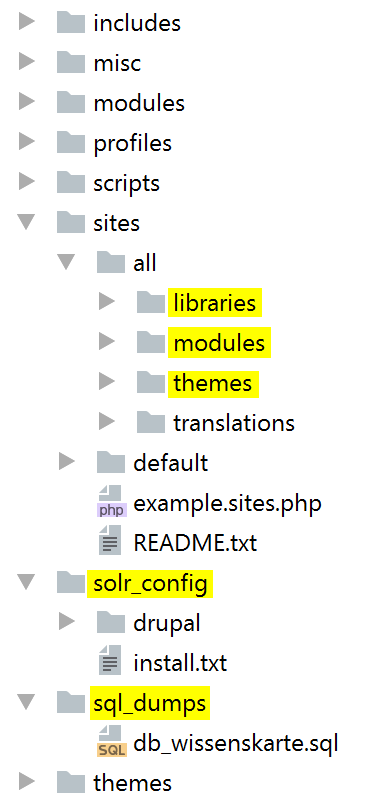
\includegraphics[height=0.25\textheight]{images/structure_project}
		\caption[]{Drupal-Projekt}
		\label{fig:structureproject}
	\end{subfigure}
	%
	\begin{subfigure}[A]{0.4\textwidth}
		\centering
		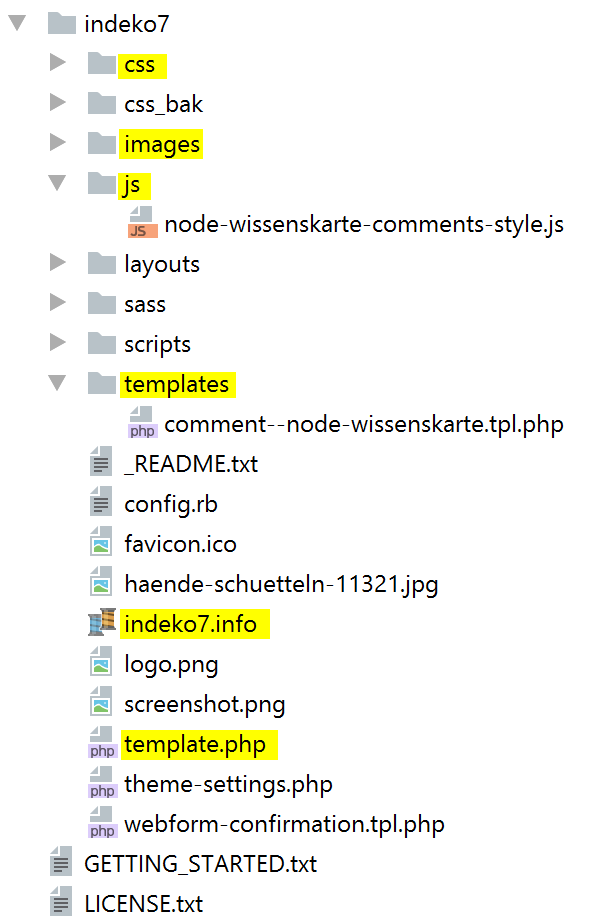
\includegraphics[height=0.25\textheight]{images/structure_theme}
		\caption[]{indeko7 Theme}
		\label{fig:structuretheme}
	\end{subfigure}
	\caption[]{Grundstruktur}
	\label{fig:structure}
\end{figure}


\cref{fig:structureproject} stellt die grundsätzliche Struktur des Drupal-Projekts dar:
\begin{itemize}
	\item \lstinline|libraries|: Enthält zusätzlich installierte externe Javascript Bibliotheken (z.B. Chosen, qTip2).
	
	\item \lstinline|modules|: Der Unterordner \lstinline|custom| enthält alle entwickelten Module.
	
	\item \lstinline|themes|: Enthält alle installiertes Drupal-Themes. Für das Projekt relevant ist das adaptivetheme indeko7 (siehe \cref{fig:structuretheme}).
	
	\item \lstinline|solr_config|: Enthält Konfigurationsdateien für den Apache Solr Server. \lstinline|install.txt| beschreibt die Installation im Detail.
	
	\item \lstinline|sql_dumps|: Enthält den Datanbank-Dump des InDeKo.Navi Atlas Projekts  (\lstinline|db_wissenskarte.sql|).
\end{itemize}


\cref{fig:structuretheme} stellt die Hauptstruktur des indeko7 Themes dar (\lstinline|\sites\all\themes\adaptivetheme\indeko7|):
\begin{itemize}
	\item \lstinline|css|: Enthält .css Dateien, die das grundlegende Design betreffen. Alle das Portal betreffenden Änderungen sind in der Datei \lstinline|global.atlas.css| zusammengefasst.
	
	\item \lstinline|images|: Der Unterordner \lstinline|atlas| enthält Bilddateien, die speziell für das Atlas-Projekt entworfen wurden und in den .css Dateien verwendet werden (z.B. spezifische Icons für Inhaltstypen oder Aktionen).
	
	\item \lstinline|js|: Enthält .js Dateien, die ausschließlich das Design betreffen. 
	
	\item \lstinline|templates|: Enthält Template-Dateien (.tpl.php), die gezielt die Darstellung der Inhalte des Portals steuern.
	
	\item \lstinline|indeko7.info|: Enthält einen zusätzlichen Eintrag, um \lstinline|global.atlas.css| einzubinden (\lstinline|stylesheets[screen][] = css/global.atlas.css|).
	
	\item \lstinline|template.php|: Enthält Logik, die die von Drupal bereitgestellten Informationen zur Darstellung der Inhalte anpasst.
	
\end{itemize}



\subsection{Grundsätzliche Modulstruktur}\label{sub:strukture_module}
\begin{figure}
	\centering
	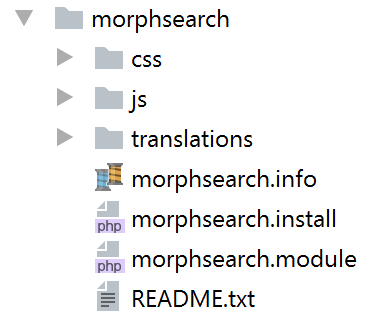
\includegraphics[height=0.2\textheight]{images/structure_module}
	\caption[]{Struktur Modul}
	\label{fig:structuremodule}
\end{figure}

Dieser Abschnitt beschreibt die grundsätzliche Struktur der entwickelten Custom Module (\lstinline|\sites\all\modules\custom|):

\begin{itemize}
	\item \lstinline|css|: Enthält .css Dateien, die speziell das Modul betreffen.
	
	\item \lstinline|js|: Enthält .js Dateien, die speziell das Modul betreffen.
	
	\item \lstinline|translations|: Enthält eine Übersetzungs-Vorlage (.pot), die alle übersetzbaren Texte des Moduls enthält und eine deutsche Übersetzungsdatei (.de.po). Die Übersetzungen werden während der Installation des Moduls importiert oder können jederzeit manuell in Drupal importiert werden (\lstinline|admin/config/regional/translate/import|). Templates erstellt mit dem Translation template extractor Modul (\url{https://www.drupal.org/project/potx})
	
	\item \lstinline|.info|: 
	
	\item \lstinline|.install|: Enthält Installations- und Deinstallationsroutinen (Variablen, Datenbank-Tabellen und Einträge).
	
	\item \lstinline|.module|: 
	
	\item \lstinline|README.txt|: Enthält die Beschreibung des Moduls, die Installationsanleitung inklusive Pflicht- und optionaler Module, sowie eine Beschreibung der Konfiguration (in Anlehnung an das Drupal README Template \url{https://www.drupal.org/node/2181737}).
\end{itemize}




\section{Anmerkungen zum Produktivbetrieb}\label{sec:live}
Dieser Abschnitt enthält Punkte, die bei der Überführung des InDeKo.Navi-Portals aus der Test-Umgebung in eine Live-Umgebung beachtet werden sollten.

\begin{itemize}
	\item In der Entwicklung genutzte Benutzeraccounts deaktivieren, da die Passwörter unsicher sind (\lstinline|admin/people|): \enquote{admin}, \enquote{ruser}, \enquote{ruser2}, \enquote{ruser3}, \enquote{ruser4}, \enquote{ruser5}.
	
	\item Beispiel-Wissenskarten löschen, da nicht geprüft wurde, ob die verwendeten Bilder lizenzfrei sind (\lstinline|admin/content|).
	
	\item Für den CSV-Export der Suchergebnisse, die aus dem Internet erreichbare URL des Apache Solr Servers eintragen (\lstinline|admin/config/morphsearch_csv_export|).
	
	\item Anzuzeigende Fehlermeldungen deaktivieren (\lstinline|admin/config/development/logging|).
\end{itemize}



\section{Funktionalität}\label{sec:function}
Dieses Kapitel beschreibt die im Laufe des Projekts entwickelten Funktionalitäten. \cref{sub:custom_modules} beschäftigt sich mit den entstandenen Custom Modulen. \cref{sub:drupal_customizing} beschreibt Funktionalitäten, die ausschließlich durch den Einsatz von Contributed oder Drupal-Core Modulen umgesetzt wurden.



\subsection{Entwickelte Custom Module}\label{sub:custom_modules}
\begin{figure}[!h]
	\centering
	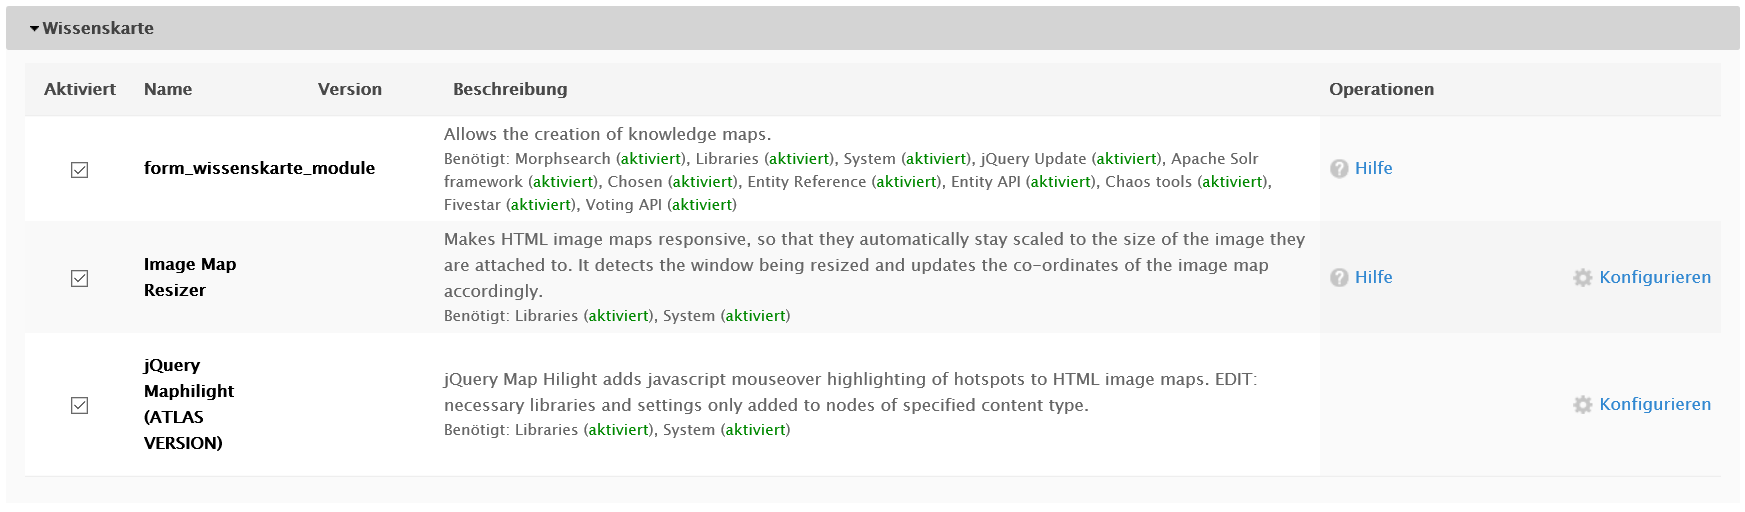
\includegraphics[width=0.8\linewidth]{images/modules_knowledgemap}
	\caption[]{Module Wissenskarte}
	\label{fig:modules_knowledgemap}
\end{figure}
\begin{figure}[!h]
	\centering
	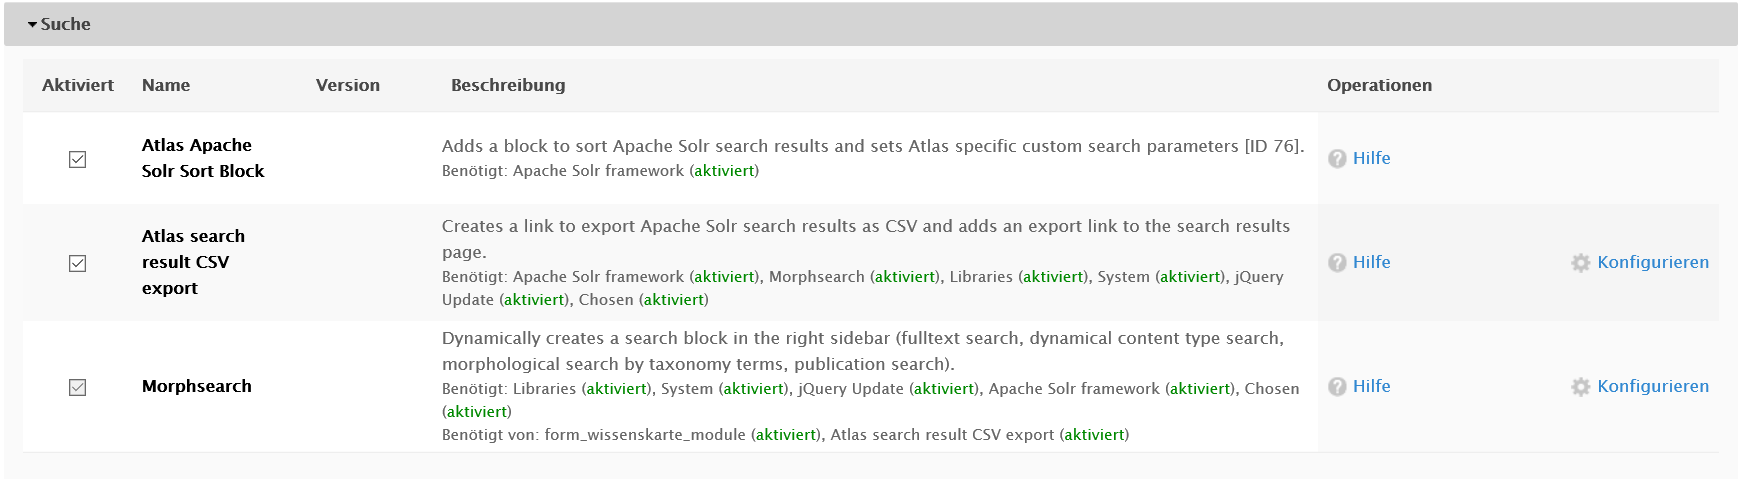
\includegraphics[width=0.8\linewidth]{images/modules_search}
	\caption[]{Module Suche}
	\label{fig:modules_search}
\end{figure}
\begin{figure}[!h]
	\centering
	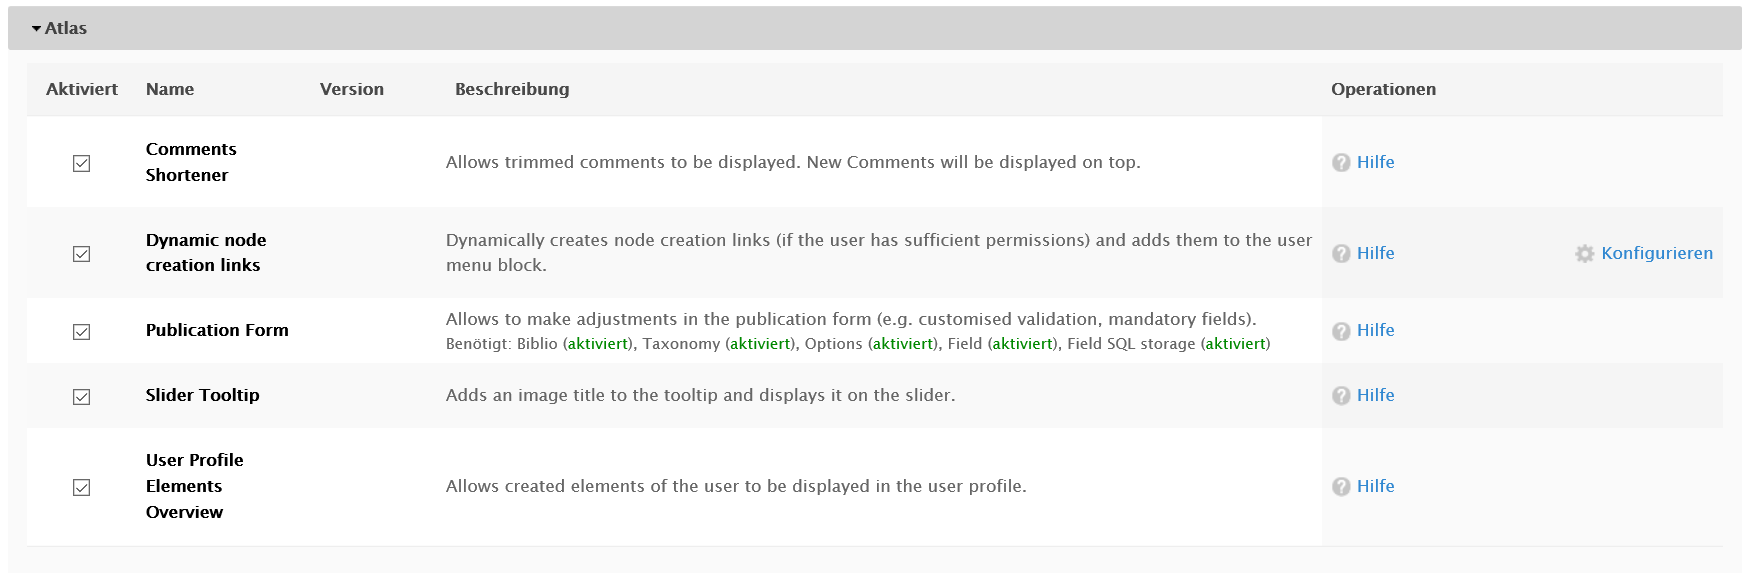
\includegraphics[width=0.8\linewidth]{images/modules_atlas}
	\caption[]{Module Atlas}
	\label{fig:modules_atlas}
\end{figure}




\subsubsection{form\_wissenskarte\_module}\label{subsub:km}
form\_wissenskarte\_module
Beschreibung, Installation, Konfiguration, vorausgesetzte Module? Sollte alles in den README.txt Dateien stehen.

\subsubsection{comments\_shortener}\label{subsub:commentsshortener}
comments\_shortener
\begin{figure}[H]
	\centering
	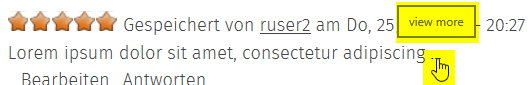
\includegraphics[width=0.50\linewidth]{images/example_commentsshortener}
	\caption[]{Beispiel comments\_shortener}
	\label{fig:example_commentshortener}
\end{figure}



\subsubsection{imagemap\_resizer}\label{subsub:imagemapresizer}
imagemap\_resizer
\begin{figure}[H]
	\centering
	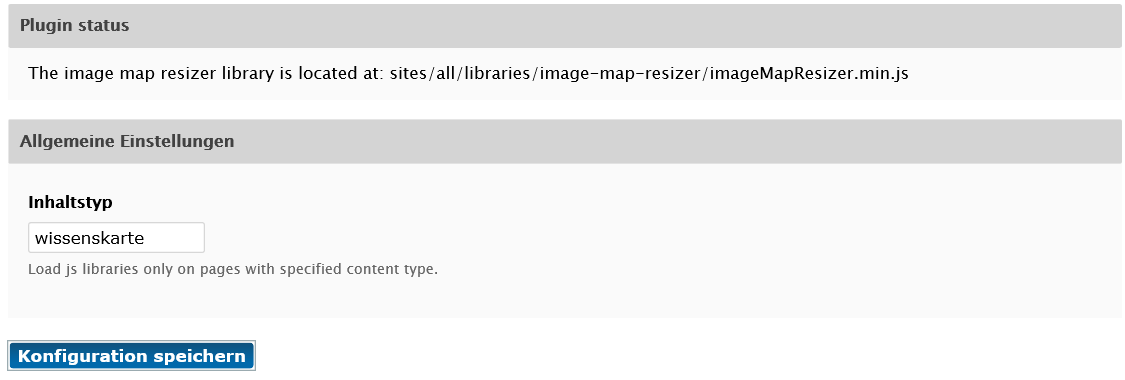
\includegraphics[width=0.70\linewidth]{images/config_imagemapresizer}
	\caption[]{Konfigurationsmenü imagemap\_resizer}
	\label{fig:config_imagemapresizer}
\end{figure}



\subsubsection{jq\_maphilight}\label{subsub:maphilight}
jq\_maphilight
\begin{figure}[H]
	\centering
	\begin{subfigure}[a]{0.4\textwidth}
		\centering
		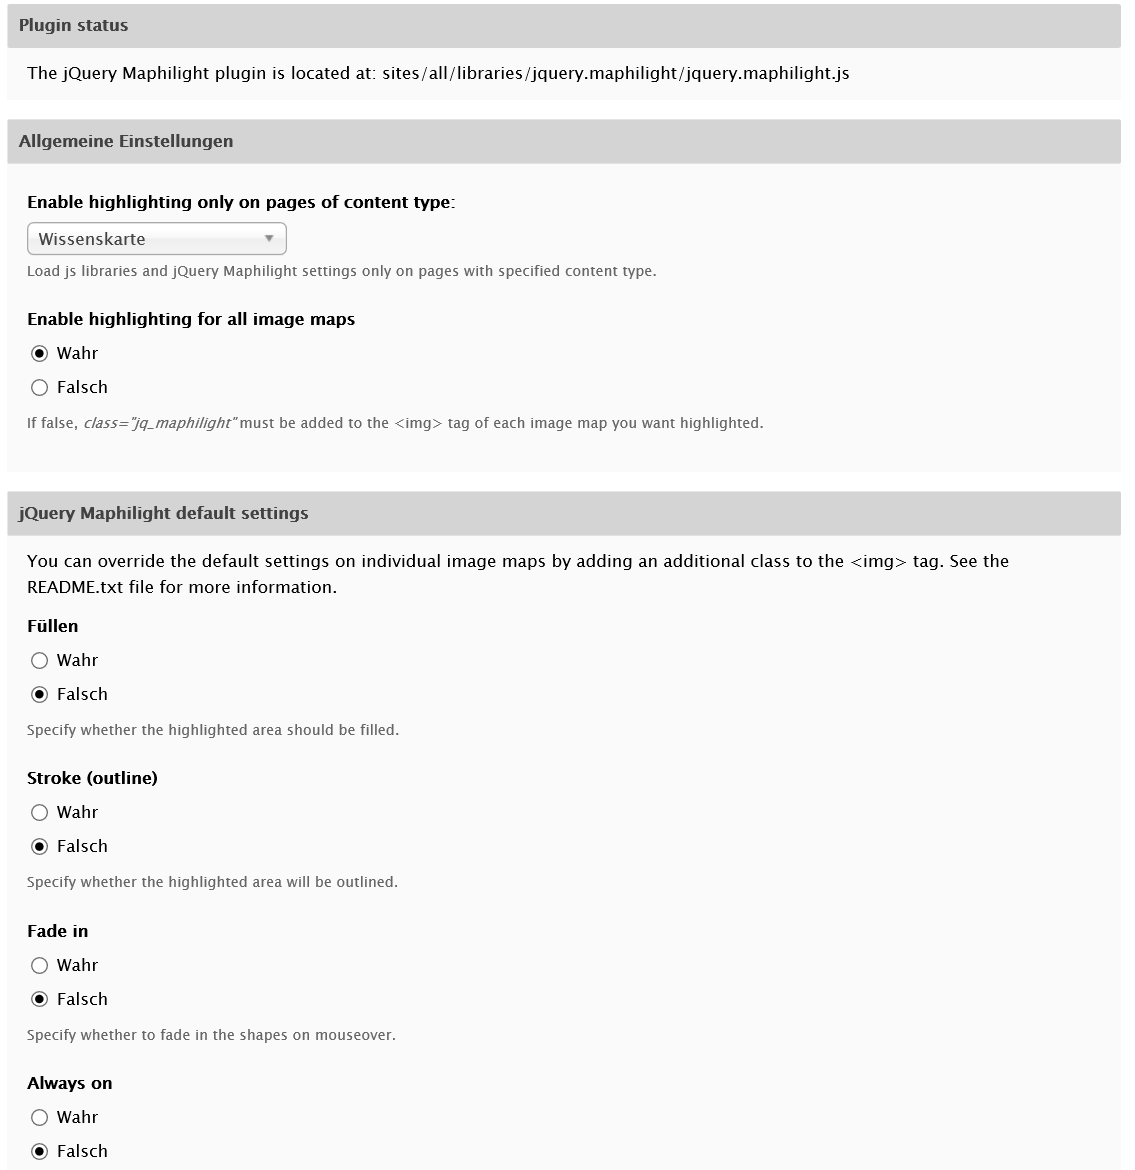
\includegraphics[height=0.20\textheight]{images/config_maphilight1}
		\caption[]{Allgemeine Einstellungen}
		\label{fig:config_maphilight1}
	\end{subfigure}
	%
	\begin{subfigure}[A]{0.4\textwidth}
		\centering
		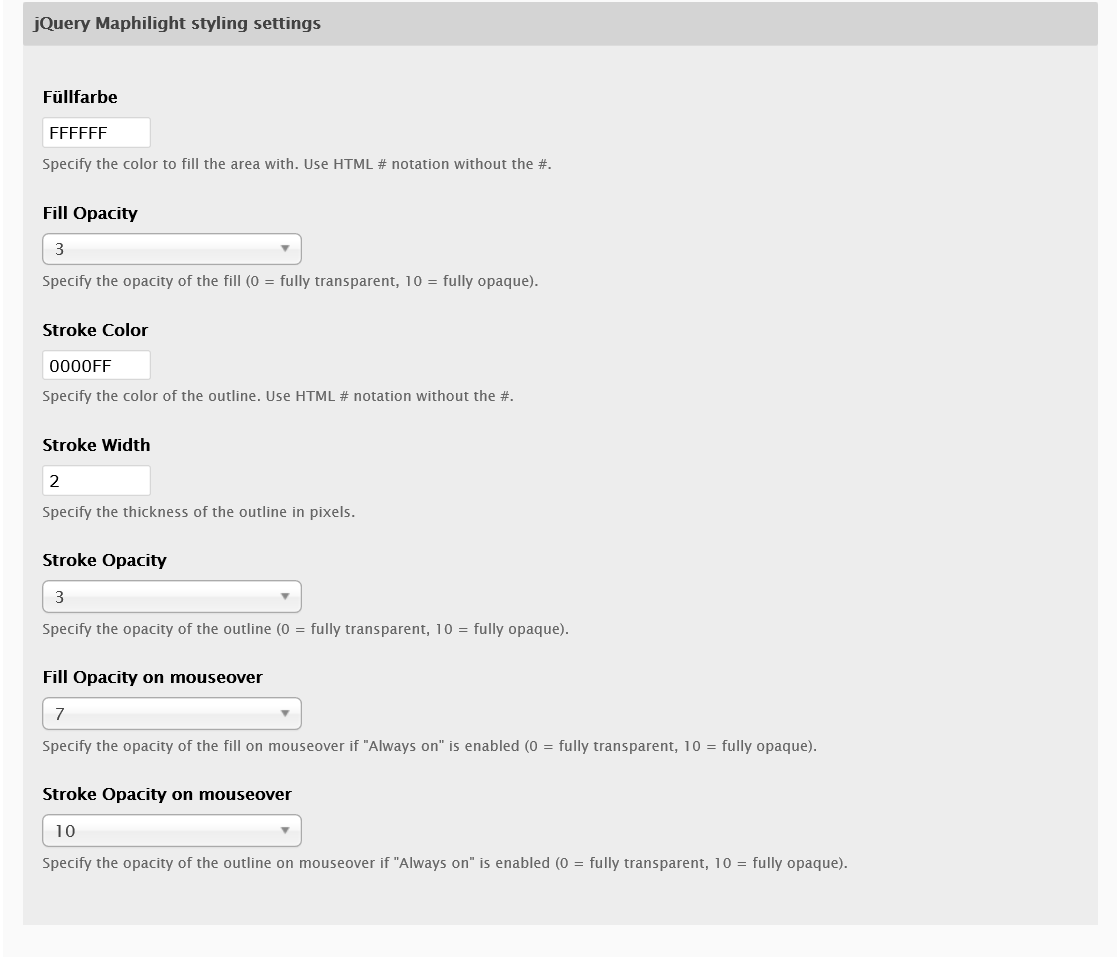
\includegraphics[height=0.20\textheight]{images/config_maphilight2}
		\caption[]{Styling Einstellungen}
		\label{fig:config_maphilight2}
	\end{subfigure}
	\caption[]{Konfigurationsmenü jq\_maphilight}
	\label{fig:config_maphilight}
\end{figure}




\subsubsection{morphsearch}\label{subsub:morphsearch}
morphsearch
\begin{figure}[H]
	\centering
	\begin{subfigure}[a]{0.4\textwidth}
		\centering
		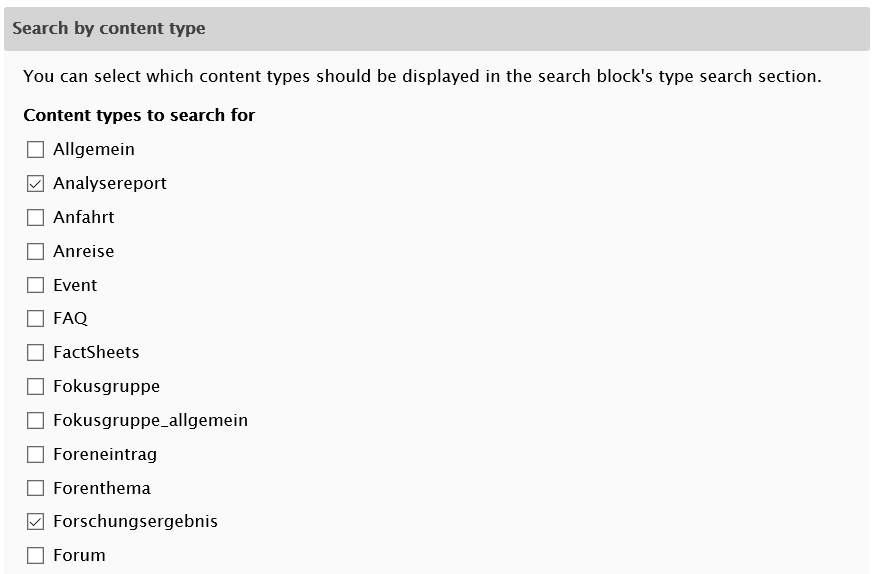
\includegraphics[height=0.20\textheight]{images/config_morphsearch}
		\caption[]{Konfigurationsmenü}
		\label{fig:config_morphsearch}
	\end{subfigure}
	%
	\begin{subfigure}[A]{0.4\textwidth}
		\centering
		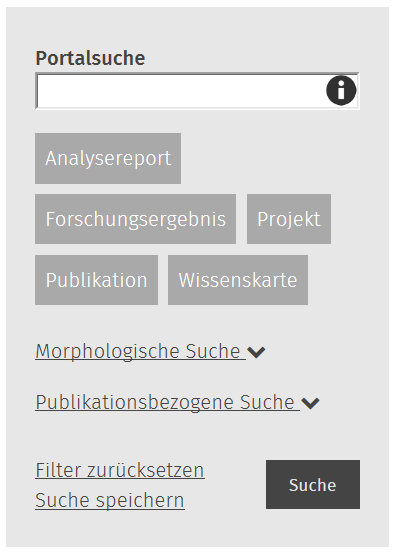
\includegraphics[height=0.20\textheight]{images/example_morphsearch}
		\caption[]{Beispiel}
		\label{fig:example_morphsearch}
	\end{subfigure}
	\caption[]{morphsearch}
	\label{fig:morphsearch}
\end{figure}



\subsubsection{morphsearch\_csv\_export}\label{subsub:morphsearchcsv}
morphsearch\_csv\_export
\begin{figure}[H]
	\centering
	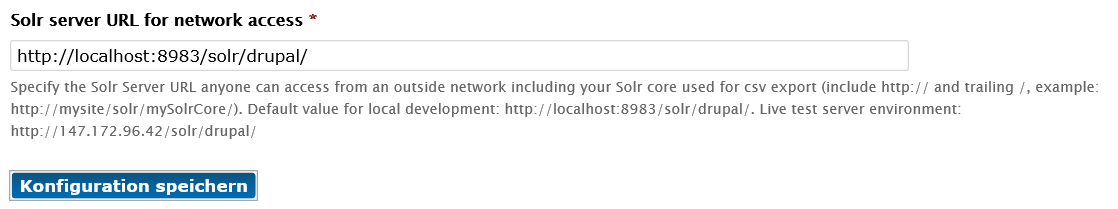
\includegraphics[width=0.70\linewidth]{images/config_searchcsv}
	\caption[]{Konfigurationsmenü morphsearch\_csv\_export}
	\label{fig:config_search}
\end{figure}



\subsubsection{morphsearch\_sort}\label{subsub:morphsearchsort}
morphsearch\_sort
\begin{figure}[H]
	\centering
	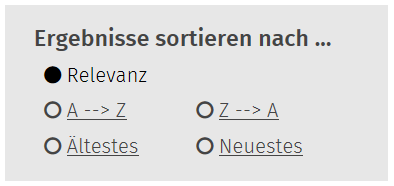
\includegraphics[height=0.10\textheight]{images/example_morphsearchsort}
	\caption[]{Konfigurationsmenü morphsearch\_sort}
	\label{fig:morphsearchsort}
\end{figure}


\subsubsection{node\_creation\_links}\label{subsub:nodecreationlinks}
node\_creation\_links
\begin{figure}[H]
	\centering
	\begin{subfigure}[a]{0.4\textwidth}
		\centering
		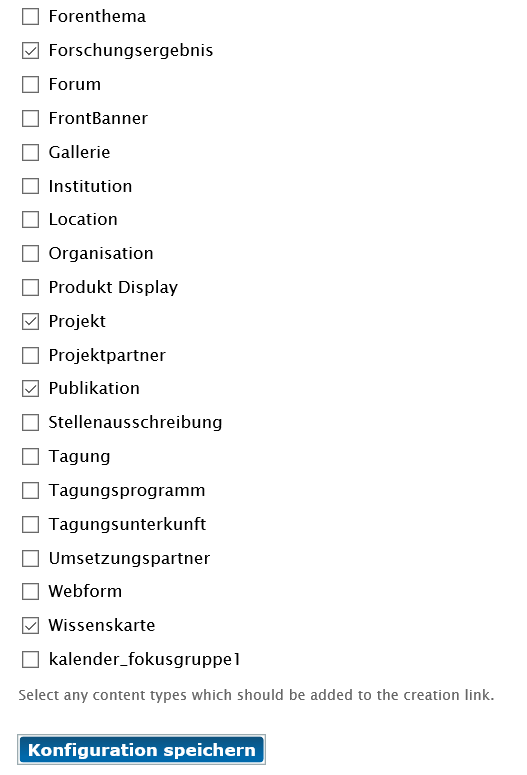
\includegraphics[height=0.20\textheight]{images/config_nodecreationlinks}
		\caption[]{Konfigurationsmenü}
		\label{fig:config_nodecreationlinks}
	\end{subfigure}
	%
	\begin{subfigure}[A]{0.4\textwidth}
		\centering
		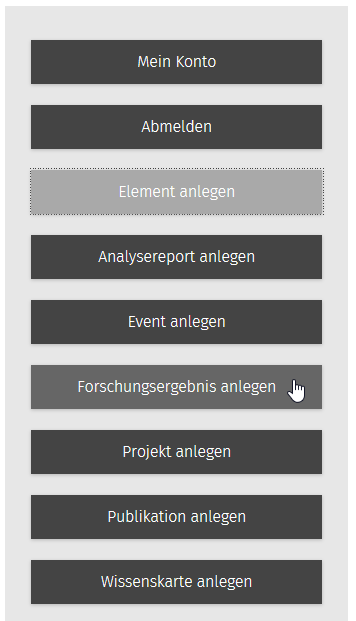
\includegraphics[height=0.20\textheight]{images/example_nodecreationlinks}
		\caption[]{Beispiel}
		\label{fig:example_nodecreationlinks}
	\end{subfigure}
	\caption[]{node\_creation\_links}
	\label{fig:nodecreationlinks}
\end{figure}



\subsubsection{publication\_form}\label{subsub:publicationform}
publication\_form


\subsubsection{slider\_tooltip}\label{subsub:slidertooltip}
slider\_tooltip
\begin{figure}[H]
	\centering
	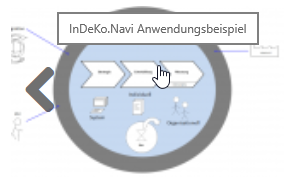
\includegraphics[height=0.10\textheight]{images/example_slidertooltip}
	\caption[]{slider\_tooltip}
	\label{fig:example_slidertooltip}
\end{figure}


\subsubsection{user\_profile\_elements\_overview}\label{subsub:userprofileelementsoverview}
user\_profile\_elements\_overview
\begin{figure}[H]
	\centering
	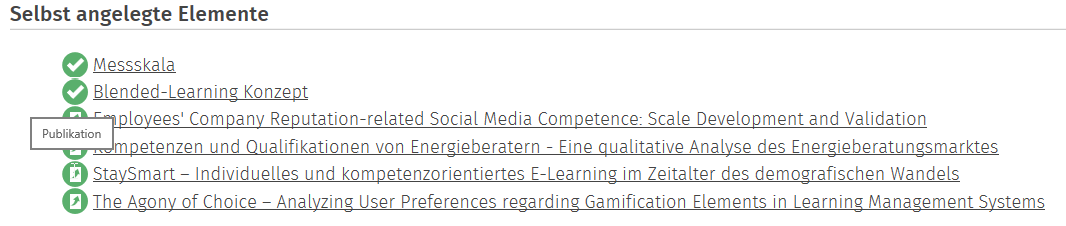
\includegraphics[width=0.80\linewidth]{images/example_userprofile}
	\caption[]{user\_profile\_elements\_overview}
	\label{fig:example_userprofile}
\end{figure}


\subsection{Drupal Customizing}\label{sub:drupal_customizing}


\subsubsection{Darstellung der Suchergebnisse}\label{subsub:suchergebnisse}
Darstellung der Suchergebnisse
\begin{figure}[H]
	\centering
	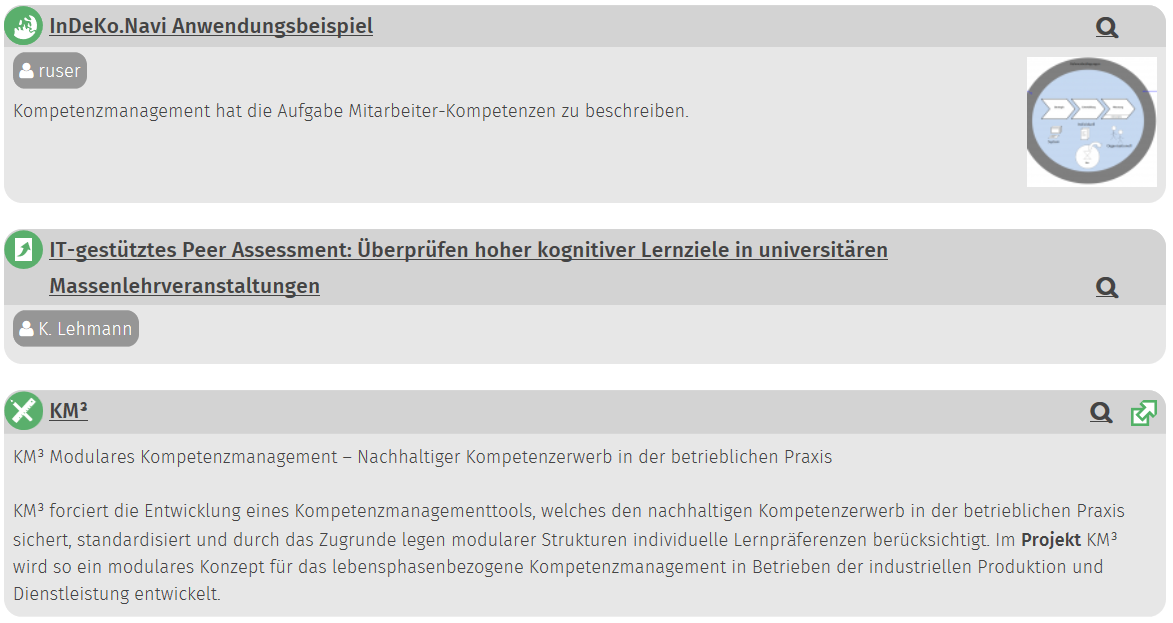
\includegraphics[height=0.20\textheight]{images/example_searchresult}
	\caption[]{Darstellung der Suchergebnisse}
	\label{fig:example_searchresult}
\end{figure}


\subsubsection{Slider mit Wissenskarten als Startseite}\label{subsub:wkslider}
Slider mit Wissenskarten als Startseite
\begin{figure}[H]
	\centering
	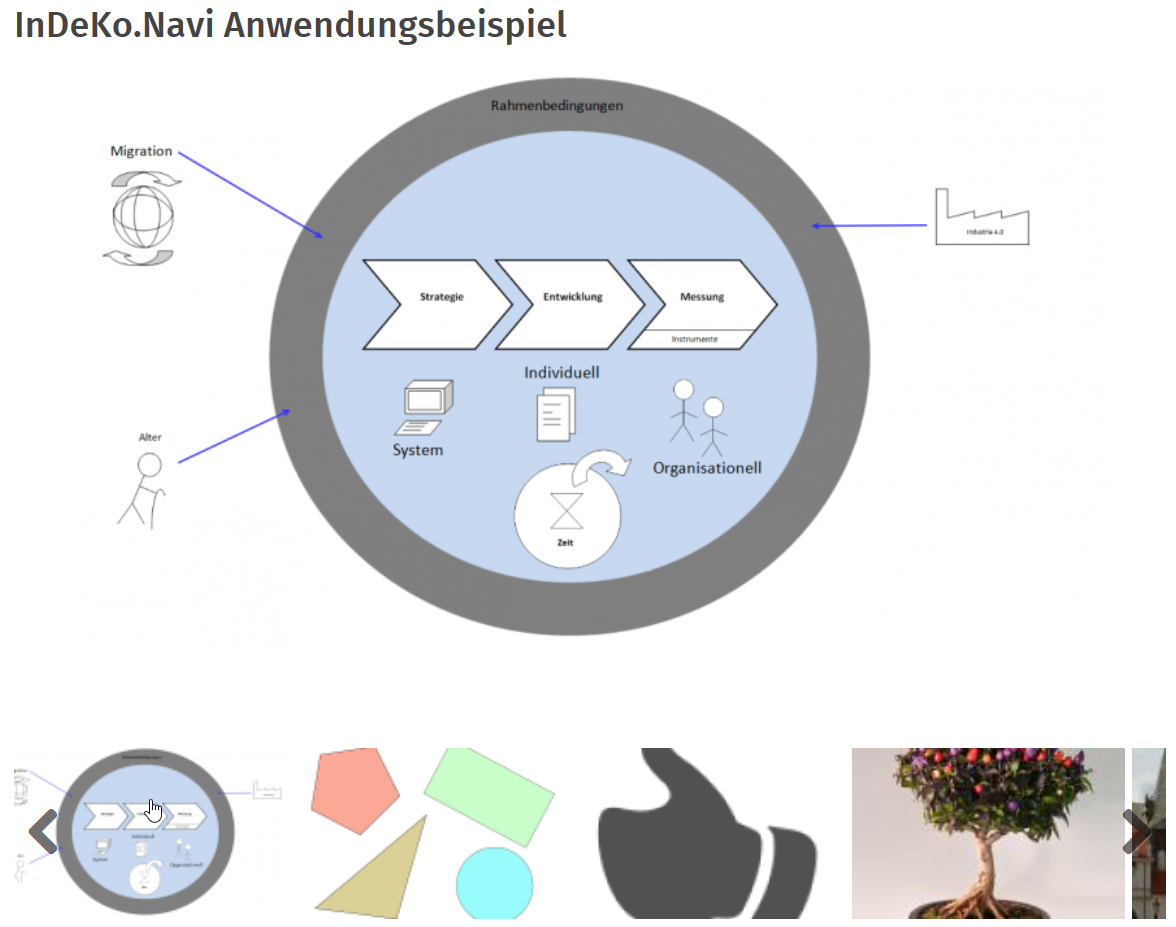
\includegraphics[height=0.20\textheight]{images/example_slider}
	\caption[]{Slider mit Wissenskarten als Startseite}
	\label{fig:example_slider}
\end{figure}

\subsubsection{CSS / Design / ???}\label{subsub:cssdesign}
CSS / Design / ???



\section{Fehler und deren Lösungen}\label{sec:problems}

\begin{itemize}
	\item \textit{ERROR 2006 (HY000) at line [...]: MySQL server has gone away}
	
	MySQL Konfiguration (my.ini | XAMPP -> MySQL -> Config)
	\textbf{max\_allowed\_packet} erhöhen (z.B. auf 32M).
	
	
	\item \textit{Fatal error: Allowed memory size of [...] bytes exhausted (tried to allocate [...] bytes) in [...]}
	
	PHP Konfiguration (php.ini | XAMPP -> Apache -> Config)
	\textbf{memory\_limit} hochsetzen .
	
	
	\item \textit{PDOException: SQLSTATE[HY000] [2002] Es konnte keine Verbindung hergestellt werden, da der Zielcomputer die Verbindung verweigerte. in lock\_may\_be\_available()}
	
	MySQL Server nicht gestartet oder abgestürzt.
	
	
	\item \textit{PDOException: SQLSTATE[42000]: Syntax error or access violation: 1118 The size of BLOB/TEXT data inserted in one transaction is greater than 10\% of redo log size. Increase the redo log size using innodb\_log\_file\_size.}
	
	MySQL Konfiguration (my.ini | XAMPP -> MySQL -> Config)
	\textbf{innodb\_log\_file\_size} erhöhen.
	
	
	\item \textit{Warning: file\_get\_contents(): http:// wrapper disabled in the server configuration by allow\_url\_fopen=0 in \_local\_parse\_js\_file()}
	
	Drupal Konfiguration zur settings.php \textbf{ini\_set('allow\_url\_fopen', 1);} hinzufügen.
	
	
	\item
		
	
\end{itemize}


\section{Offene Punkte}


\section{Glossar}\label{sec:glossary}




\newpage
\printbibliography
%\bibliography{atlas}
\end{document}